% +-------------------------------------------------------------------------+
% | INSTITUTO FEDERAL DO PARANÁ                                             |
% | Título: Artigo acadêmico                                                |
% | Prof. Dr. Jiusandro Kuhn                                                |
% | jiusandro.kuhn@ifpr.edu.br                                              |
% +-------------------------------------------------------------------------+
%
% +-------------------------------------------------------------------------+
% | LICENÇA                                                                 |
% | Licença Creative Commons                                                |
% | Este trabalho está licenciado com uma Licença Creative Commons          |
% | Atribuição 4.0 Internacional.                                           |
% | Dr. Jiusandro Kuhn - www.jiusandro.com - jiusandro@gmail.com            |
% +-------------------------------------------------------------------------+
%
% +-------------------------------------------------------------------------+
% | INFORMAÇÕES                                                             |
% | Esse modelo de trabalho acadêmico possui a seguinte estrutura:          |
% | PRINCIPAL                                                               |
% |    artigo                                                               |
% | ELEMENTOS PRÉ-TEXTUAIS                                                  |
% |    título                      (obrigatório - via comando LaTeX)        |
% |    autor(res)                  (obrigatório - via comando LaTeX)        |
% |    data                        (obrigatório - via comando LaTeX)        |
% |    instituição/departamento    (opcional)                               |
% |    resumo                      (obrigatório)                            |
% |    sumário                     (opcional - via comando LaTeX)           |
% | ELEMENTOS TEXTUAIS                                                      |
% |    introducao                  (obrigatório)                            |
% |    desenvolvimento             (obrigatório)                            |
% |    conclusão                   (obrigatório)                            |
% |    agradecimentos              (opcional)                               |
% | ELEMENTOS PÓS-TEXTUAIS                                                  |
% |    apendice_a                  (opcional)                               |
% |    referencias bibliográficas  (obrigatório - via comando LaTeX)        |
% +-------------------------------------------------------------------------+
\documentclass[%
a4paper, % Formato do papel
twocolumn, % Duas colunas
10pt % Tamanho da fonte Opções: 10pt, 11pt
]{article}
%
% +---------+
% | Pacotes | 
% +---------+
% PACOTES BÁSICOS
\usepackage{lmodern} % Usa a fonte Latin Modern			
\usepackage[T1]{fontenc}	 % Selecao de codigos de fonte
\usepackage[utf8]{inputenc} % Codificacao do documento (conversão automática dos acentos)
\usepackage{indentfirst}	 % Indenta o primeiro parágrafo de cada seção
\usepackage{color} % Controle das cores
\usepackage{graphicx} % Inclusão de figuras
\usepackage{microtype} % para melhorias de justificação
% PACOTES ADICIONAIS
\usepackage{lipsum} % Para geração de dummy text
\usepackage{abstract} % Ajuste do resumo do artigo
\usepackage{natbib} % Referência bibliogáfica semelhante (não igual) a abnt
% PACOTE DE INTERNACIONALIZAÇÃO (BRAZIL)
\usepackage[brazil]{babel}
\usepackage{fancyhdr} % Decoração da página
%
% +-----------------------------------------------+
% | LAYOUT DO ARTIGO                              |
% | Dimensionamento das margens da página.        |
% +-----------------------------------------------+
\setlength{\oddsidemargin}{0cm} % Margem Esquerda
\setlength{\textwidth}{16cm} % Largura do Texto (Margem Direita)
\setlength{\topmargin}{0cm} % Margem Superior
\setlength{\textheight}{23cm} % Página do Texto
\setlength{\parindent}{0.8cm} % Tamanho do paragrafo
\setlength{\footskip}{1cm} % Rodapé
\setlength{\skip\footins}{7mm} % Fim do texto / inicio do rodapé
%\renewcommand{\baselinestretch}{1.5} % Descomente para colocar espaço 1.5
%
% +-----------------------------------------------+
% | INFORMAÇÕES GERAIS                            |
% | Informações e dados para composição do artigo |
% +-----------------------------------------------+
\pagestyle{fancy} % Não retirar (Para colocar decoração)
\fancyhead[RO]{Nome da disciplina}
\fancyhead[LO]{\textsc{Instituto Federal do Paraná}}
\title{\textbf{Modelo de artigo acadêmico}}
\author{Carlos José Pereira, João da Silva e Maria Cristina da Rosa\\
Instituto Federal do Paraná\\
email:\texttt{jiusandro.kuhn\@ifpr.edu.br}
}
\date{\textit{Paranaguá,\today}}
%
% +---------------------+
% | INÍCIO DO DOCUMENTO |
% +---------------------+
\begin{document}
\twocolumn[ % INÍCIO: Comando para ajuste dos elementos pré-textuais em uma coluna
\begin{@twocolumnfalse}

% ===================================-===================================
% ----------------------- ELEMENTOS PRÉ-TEXTUAIS ------------------------
% =======================================================================
\maketitle
\thispagestyle{fancy}

% +--------+
% | RESUMO |
% +--------+
\begin{abstract}
Nam dui ligula, fringilla a, euismod sodales, sollicitudin vel, wisi. Morbi auctor lorem non justo. Nam lacus libero, pretium at, lobortis vitae, ultricies et, tellus. Donec aliquet, tortor sed accumsan bibendum, erat ligula aliquet magna, vitae ornare odio metus a mi. Morbi ac orci et nisl hendrerit mollis. Suspendisse ut massa. Cras nec ante. Pellentesque a nulla. Cum sociis natoque penatibus et magnis dis parturient montes, nascetur ridiculus mus. Aliquam tincidunt urna. Nulla ullamcorper vestibulum turpis. Pellentesque cursus luctus mauris.
\end{abstract}

\end{@twocolumnfalse}
] % FIM: Comando para ajuste dos elementos prét-textuais em uma coluna

% +---------+
% | SUMÁRIO |
% +---------+
\tableofcontents % Comente esta linha para não gerar sumário

% ===================================-===================================
% ------------------------ ELEMENTOS TEXTUAIS ---------------------------
% =======================================================================

% +--------------------------+
% | INTRODUÇÃO (Obrigatório) |
% +--------------------------+
\section{Introdução}
Lorem ipsum dolor sit amet, consectetur adipiscing elit. Sed mollis ligula augue, eget rutrum lectus auctor eget. Class aptent taciti sociosqu ad litora torquent per conubia nostra, per inceptos himenaeos. Cras lacinia dapibus eros, a auctor enim semper sit amet. Aenean quis arcu scelerisque, scelerisque lorem et, luctus nisl. Nunc malesuada velit id neque auctor pretium. Cras scelerisque pretium mi, vel viverra est porttitor vitae. Nam arcu magna, vehicula sed libero sed, tempor consequat lorem. Nam vitae lectus sollicitudin, sodales nulla ac, consequat eros. Integer pharetra pellentesque dolor id pharetra. Nunc aliquet efficitur blandit. Refs.~\citep{gil2010,oliveira2011,calcada2005}.

\begin{table*}[htb]
\centering
\begin{tabular}{c c c c c c} \hline \hline
Item & Pellentesque & tristique &  habitasse & Phasellus & sapien\\
     & Coluna A1 (mm) & Coluna A2 (mm) & Coluna B1 (mm) & Coluna B2 (mm) & Coluna C1 \\
 & $\pm$ 0,5 & $\pm$ 0,5 & $\pm$ 0,5 & $\pm$ 0,5 & $\pm$ 0,5  \\ \hline
1 & 23 & 99 & 21 & 41 & 208 \\
2 & 21 & 90 & 18 & 33 & 190 \\
3 & 10 & 23 & 16 & 26 & 290 \\ 
4 & 8 &  12 & 18 & 98 & 312 \\
5 & 6 & 27 & 12 & 30 & 111 \\ 
6 & 4 & 29 & 10 & 32 & 298 \\ \hline \hline
\end{tabular}
\caption{\label{tabela2}Maecenas eu gravida ante. Curabitur at porttitor nisi, nec efficitur arcu. Nunc sollicitudin rutrum volutpat. Suspendisse vel ipsum blandit enim porta tempor.}
\end{table*}

Pellentesque sit amet est quis est dignissim volutpat. Phasellus porta lacus velit, sed rhoncus magna scelerisque et. Aliquam at sapien at augue viverra ultrices. Praesent efficitur nisi nulla, nec sodales purus fermentum et. Mauris faucibus pulvinar ipsum, sed ultricies ex bibendum sed. Donec dapibus mauris eu lorem porta, vitae bibendum sapien rutrum. Nullam congue sapien scelerisque est consequat tincidunt. Vestibulum at accumsan mi, ac molestie nisl. Aenean a quam in justo dapibus blandit. Nam eu porta tortor, ac viverra justo. Vivamus mollis urna malesuada dolor egestas lacinia.

In hac habitasse platea dictumst. Mauris mauris sem, aliquam rutrum lacus sit amet, finibus blandit nisi. Integer sed odio urna. Etiam consequat quis ante quis tristique. Donec tortor mauris, porttitor id neque a, hendrerit ornare massa. Vestibulum vel scelerisque nulla. Quisque nec urna quis ex sollicitudin ornare eget eu massa. Pellentesque habitant morbi tristique senectus et netus et malesuada fames ac turpis egestas. Nam scelerisque mattis elit, nec rhoncus ipsum luctus sed. Integer in justo nec diam tempor euismod. Suspendisse potenti. Nulla bibendum vitae elit eu facilisis.

Cum sociis natoque penatibus et magnis dis parturient montes, nascetur ridiculus mus. Suspendisse potenti. Nam accumsan erat in est aliquam cursus. Etiam lacinia sapien nibh, eu tempor turpis efficitur eget. Proin feugiat eu massa non aliquam. Vivamus et euismod sapien. Aenean eget ante eu sem fermentum vehicula sed in sapien. Curabitur porttitor semper urna vestibulum eleifend. Aenean vitae odio ultricies, congue lacus non, pellentesque quam. Quisque egestas tortor et libero porta, sit amet viverra enim mattis. Suspendisse lobortis suscipit quam, id aliquam lorem facilisis nec. 

Nulla malesuada porttitor diam. Donec felis erat, congue non, volutpat at, tincidunt tristique, libero. Vivamus viverra fermentum felis. Donec nonummy pellentesque ante\footnote{Morbi dolor nulla, malesuada eu, pulvinar at, mollis ac, nulla.}. Phasellus adipiscing semper elit. Proin fermentum massa ac quam. Sed diam turpis, molestie vitae, placerat a, molestie nec, leo. Maecenas lacinia. Nam ipsum ligula, eleifend at, accumsan nec, suscipit a, ipsum. Morbi blan- dit ligula feugiat magna. Nunc eleifend consequat lorem. Sed lacinia nulla vitae enim. Pellentesque tincidunt purus vel magna. Integer non enim. Praesent euismod nunc eu purus. Donec bibendum quam in tellus. Nullam cursus pulvinar lectus. Donec et mi. Nam vulputate metus eu enim. Vestibulum pellentesque felis eu massa \footnote{Nam dui ligula, fringilla a, euismod sodales, sollicitudin vel, wisi.}.


% +-------------------------------+
% | DESENVOLVIMENTO (Obrigatório) |
% +-------------------------------+
\section{Desenvolvimento}

Lorem ipsum dolor sit amet, consectetur adipiscing elit. Sed mollis ligula augue, eget rutrum lectus auctor eget. Class aptent taciti sociosqu ad litora torquent per conubia nostra, per inceptos himenaeos. Cras lacinia dapibus eros, a auctor enim semper sit amet. Aenean quis arcu scelerisque, scelerisque lorem et, luctus nisl. Nunc malesuada velit id neque auctor pretium. Cras scelerisque pretium mi, vel viverra est porttitor vitae. Nam arcu magna, vehicula sed libero sed, tempor consequat lorem. Nam vitae lectus sollicitudin, sodales nulla ac, consequat eros. Integer pharetra pellentesque dolor id pharetra. Nunc aliquet efficitur blandit. Eq.~(\ref{distr_maxwell}).

\begin{equation}
P(v) = 4\pi \left(\frac{M}{2\pi R T}\right)^{3/2} v^2 e^{-\frac{M v^2}{2RT}}
\label{distr_maxwell}
\end{equation}

Pellentesque sit amet est quis est dignissim volutpat. Phasellus porta lacus velit, sed rhoncus magna scelerisque et. Aliquam at sapien at augue viverra ultrices. Praesent efficitur nisi nulla, nec sodales purus fermentum et. Mauris faucibus pulvinar ipsum, sed ultricies ex bibendum sed. Donec dapibus mauris eu lorem porta, vitae bibendum sapien rutrum. Nullam congue sapien scelerisque est consequat tincidunt. Vestibulum at accumsan mi, ac molestie nisl. Aenean a quam in justo dapibus blandit. Nam eu porta tortor, ac viverra justo. Vivamus mollis urna malesuada dolor egestas lacinia.
\begin{figure*}[htb]
\centering
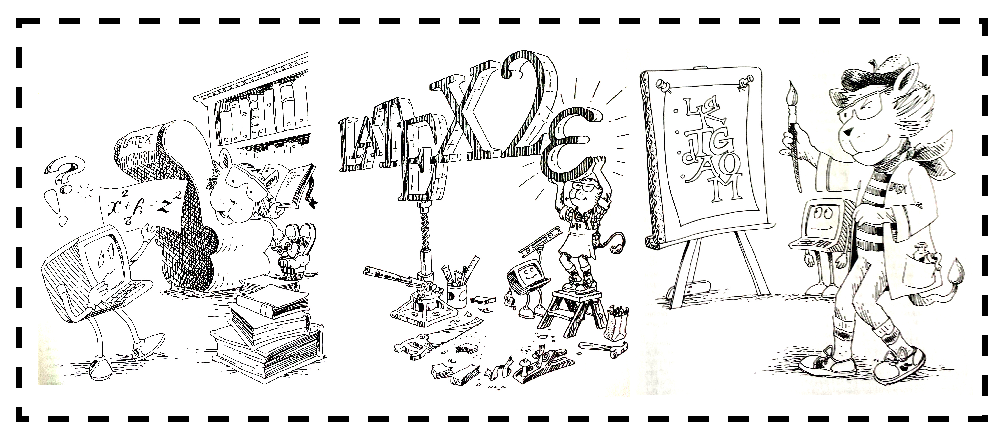
\includegraphics[width=12cm]{figura1.eps}
\caption{Fusce mi eros, molestie et purus ut, ultrices elementum eros. Nullam sed metus sollicitudin, feugiat tellus at, lacinia turpis.}
\end{figure*}

In hac habitasse platea dictumst. Mauris mauris sem, aliquam rutrum lacus sit amet, finibus blandit nisi. Integer sed odio urna. Etiam consequat quis ante quis tristique. Donec tortor mauris, porttitor id neque a, hendrerit ornare massa. Vestibulum vel scelerisque nulla. Quisque nec urna quis ex sollicitudin ornare eget eu massa. Pellentesque habitant morbi tristique senectus et netus et malesuada fames ac turpis egestas. Nam scelerisque mattis elit, nec rhoncus ipsum luctus sed. Integer in justo nec diam tempor euismod. Suspendisse potenti. Nulla bibendum vitae elit eu facilisis.

\subsection{Título da subseção}
Etiam iaculis lectus sit amet cursus gravida. Pellentesque habitant morbi tristique senectus et netus et malesuada fames ac turpis egestas. Ut pharetra ex nisl, quis auctor ante imperdiet in. Cras blandit neque at porta facilisis. Vestibulum cursus hendrerit velit consectetur aliquam. Etiam lacinia leo metus, sit amet convallis sem faucibus nec. Donec at tempus lectus. Cras dictum feugiat lorem quis dignissim. Praesent rutrum nec justo eget gravida. Sed pharetra dolor in ligula eleifend dapibus. Donec blandit elit justo, imperdiet maximus libero sagittis eget. Aenean vehicula vehicula dui, eget eleifend ex tristique egestas. Integer eu malesuada nunc. 

\subsection{Título da subseção}
 Nullam non scelerisque ligula. Vivamus suscipit tortor tortor. Quisque tempor enim vel eleifend gravida. Maecenas egestas ex eget tellus posuere, a tincidunt lacus luctus. Pellentesque dapibus cursus tincidunt. Vivamus facilisis turpis vitae dolor tincidunt molestie. Integer varius tortor in metus tincidunt tristique.

Sed vel ex ipsum. Sed id diam tristique, scelerisque arcu sit amet, rhoncus sem. Morbi vitae metus finibus, posuere quam sit amet, luctus lacus. Sed dictum ultrices enim non eleifend. Sed efficitur enim metus, sed imperdiet ante egestas in. Integer a purus sit amet massa volutpat pellentesque. Aliquam rutrum non nibh id semper. 
\begin{figure}[htb]
\centering
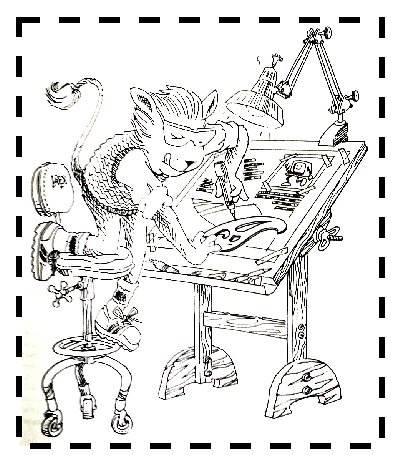
\includegraphics[width=5cm]{figura2.eps}
\caption{Mauris laoreet posuere neque, scelerisque dignissim libero tempus et.}
\end{figure}

% +-------------------------+
% | CONCLUSÃO (Obrigatório) |
% +-------------------------+
\section{Conclusão}
\lipsum[2-8]

\section*{Agradecimentos}
Morbi luctus ullamcorper libero, eu lobortis dolor rhoncus sed. Curabitur neque velit, porttitor et dignissim ut, molestie vitae erat. Aliquam efficitur ex dui, id consequat odio iaculis a. Maecenas eu gravida ante.

% ===================================-===================================
% ------------------------ ELEMENTOS PÓS-TEXTUAIS -----------------------
% =======================================================================

% +-----------+
% | APÊNDICES |
% +-----------+
\appendix
\section{Título do apêndice}
\lipsum[1-2]

% +----------------------------+
% | REFERÊNCIAS BIBLIOGRÁFICAS |
% +----------------------------+
\bibliographystyle{unsrt} % Opções: unsrt, alpha, abbrv
%\bibliographystyle{plainnat}
\bibliography{referencias}
\addcontentsline{toc}{section}{Referências} % Para incluir a referência no sumário

\end{document}